\setcounter{chaptercntr}{4}

\sectionbreak {
\gostTitleFont
\redline
\thechaptercntr . 
РАЗРАБОТКА, ОБУЧЕНИЕ И ТЕСТИРОВАНИЕ МОДЕЛИ НЕЙРОННОЙ

\redline СЕТИ
}


\titlespace

\subsection*{ 
  \gostTitleFont
  \redline
  \thechaptercntr .\thesubchaptercntr \spc 
  Выбор архитектуры нейронной сети для прогнозирования
} \addtocounter{subchaptercntr}{1} 

\subtitlespace

{\gostFont

  \par \redline Для выбора архитектуры нейронной сети необходимо для начала понять, какие архитектуры используются для прогнозирования данных временных рядов. Зачастую для выполнения данной задачи используются однослойные персептроны, многослойные персептроны и реккурентные нейронные сети. Обращая внимание на свойства данных, становится понятно, что однослойный персептрон не сможет обеспечить необходимую обобщающую способность. Тогда остаётся выбор между многослойным перспетроном и реккурентной нейронной сетью. 
  
  \par \redline Относительно многослойных персептронов существует теорема, согласно которой персептрон с одним скрытым слоем является универсальным аппроксиматором, т. е. он способен с любой степенью точности аппроксимировать любую непрерывную функцию, если в качестве функции активации нейронных элементов скрытого слоя используется непрерывная, монотонно возрастающая, ограниченная функция. При этом точность аппроксимации функции зависит от количества нейронов в скрытом слое. Чем больше количество нейронов, тем больше точность аппроксимации. Однако при слишком большой размерности скрытого слоя может наступить явление, которое называется перетренировкой сети, когда сеть имеет плохую обобщающую способность.  

  \par \redline Что касается RNN, также существует теорема, говорящая нам о том, что любая нелинейная динамическая система при использовании достаточного количества сигмоидальных нейронных элементов в скрытом слое с любой точностью может быть аппроксимирована рекуррентной нейронной сетью. 

  \par \redline Выходит, что для прогнозирования можно использовать как многослойный перспетрон, так и RNN. Однако, RNN обаладает очень интересной чертой: она обладает, так называемой, памятью, способной <<запоминать>> особенности данных временных рядов. Такой памятью многослойный персептрон не обладает. Поскольку данные имеют в себе отличающиеся друг от дурга, но повторяющиеся в будущем участки, то наличие такой памяти было бы очень кстати. Также, как можно будет узнать дальше, большинство, если не все, RNN имеют чётко определённую структуру, в которую довольно сложно что-то добавить, да и нет в этом необходимости. В случае с многослойными персептронами, их структура не постоянна: необходимо подбирать количество скрытых слоёв. Поэтому в некотором смысле, реализация RNN не только будет выгоднее, но и проще. При этом, если обратиться к Kaspersky MLAD, то можно вспомнить, что для прогнозирования данных телемпетрии используются именно RNN. Учитывая всё вышенаписанное, выбор архитектуры падает на RNN.

  \par \redline Теперь необходимо выбрать модель RNN. Существует большое количество различных реккурентных нейронных сетей: SRN Джордана, SRN Элмана, мультиреккурентная нейронная сеть, LSTM, GRU и так далее. Однако, одной из самых распространнённых и эффектовных RNN считают LSTM сеть. Эта сеть встречается куда чаще, чем её модификации, такие как GRU, MGU, LSTM <<с глазками>> и другие. Основной задачей ставилось упрощение сети без вреда её точности, результатом чего появилась ранее упомянутая GRU, точность предсказаний которой не уступает LSTM, но при этом сеть менее грамоздкая. Упростить удалось и GRU, получив тем самым MGU, однако точность этой сети всё также сравнивалась с LSTM. Поэтому для данной работы за основу будет взята классическая LSTM.

  \par \redline К слову, LSTM была выбрана и Kaspersky при разработке системы MLAD. Это в очередной раз говорит о популярности и надёжности сети LSTM, что укрепляет уверенность в выборе LSTM сети для данной работы. 

  \par
}

\subtitlespace

\subsection*{ 
  \gostTitleFont
  \redline
  \thechaptercntr .\thesubchaptercntr \spc 
  Обзор LSTM как средства прогнозирования
} \addtocounter{subchaptercntr}{1} 
  
\subtitlespace
  
{\gostFont

  \par \redline Сеть LSTM обладает двумя видами памяти, которые способны сохранять различные зависимости в данных. Есть долгосрочная память, которая обозначается как $ C_{t} $, и краткосрочная память, которая обозначается как $ H_{t} $. Как можно догадаться, долгосрочная память сети хранит в себе особенности данных на протяжении всей истории, а краткосрочная память хранит зависимости ближайших промежутков и сильнее влияет на результат прогноза. Зачастую краткосрочную память сети обозначают как её выход. При этом входом сети является некоторый вектор данных, на основании которых будет делаться прогноз. Вектор входных данных будет обозначаться как $ X_{t} $. Как можно заметить, у всех параметров сети присутствует временная компонента t. Это говорит о том, что расчёт прогноза происходит относительно времени. Каждая новая итерация сети происходит с изменением времени. Память сети изменяется на одной из итерации и передаётся на следующую, тем самым сеть и сохраняется особенности данных временного ряда, который был подан на вход сети. Такая передача памяти возможно благодаря, так называемых в нейронных сетя, обратных связях, наличие которые и определяет сеть как реккурентную. Вышеописанное можно увидеть на рисунке \thechaptercntr .\theimagecntr. 

  \begin{figure}[H]
    \centering
    \def\svgwidth{\textwidth}
    \includesvg[width=190pt]{images/LSTMBlackBox.svg}
    \caption*{\gostFont Рисунок \thechaptercntr .\theimagecntr \spc {--} Блок LSTM сеть с изображением обратных связей.}
    \label{fig:LSTMBlackBox}
  \end{figure} \addtocounter{imagecntr}{1}

  \par \redline Каждый такой блок сети LSTM, изображённый на рисунке выше, зачастую называют ячейкой LSTM. Свзять этих ячекек между собой можно гораздо лучше увидеть на развёрнутой схеме LSTM, изображённой на рисунке \thechaptercntr .\theimagecntr. 

  \begin{figure}[H]
    \centering
    \def\svgwidth{\textwidth}
    \includesvg[width=\textwidth]{images/LSTMSequence.svg}
    \caption*{\gostFont Рисунок \thechaptercntr .\theimagecntr \spc {--} Взаимосвязь ячеект LSTM в развёрнутом виде.}
    \label{fig:LSTMSequence}
  \end{figure} \addtocounter{imagecntr}{1}

  \par \redline Теперь необхомо изучить саму ячейку LSTM. Её строение престалено на рисунку \thechaptercntr .\theimagecntr. Говоря о LSTM, можно встретить специальную лексику, которая относится к описанию этой сети. К специальной лексике относятся такие понятия как: врата забывания ($F_t$), врата входа ($I_t$), врата новой памяти ($G_t$), врата выхода ($O_t$), долгосрочная память ($C_t$) и краткосрочная память ($H_t$). Разберём каждый из них по отдельности.

  \begin{sidewaysfigure}
    \centering
    \def\svgwidth{\textwidth}
    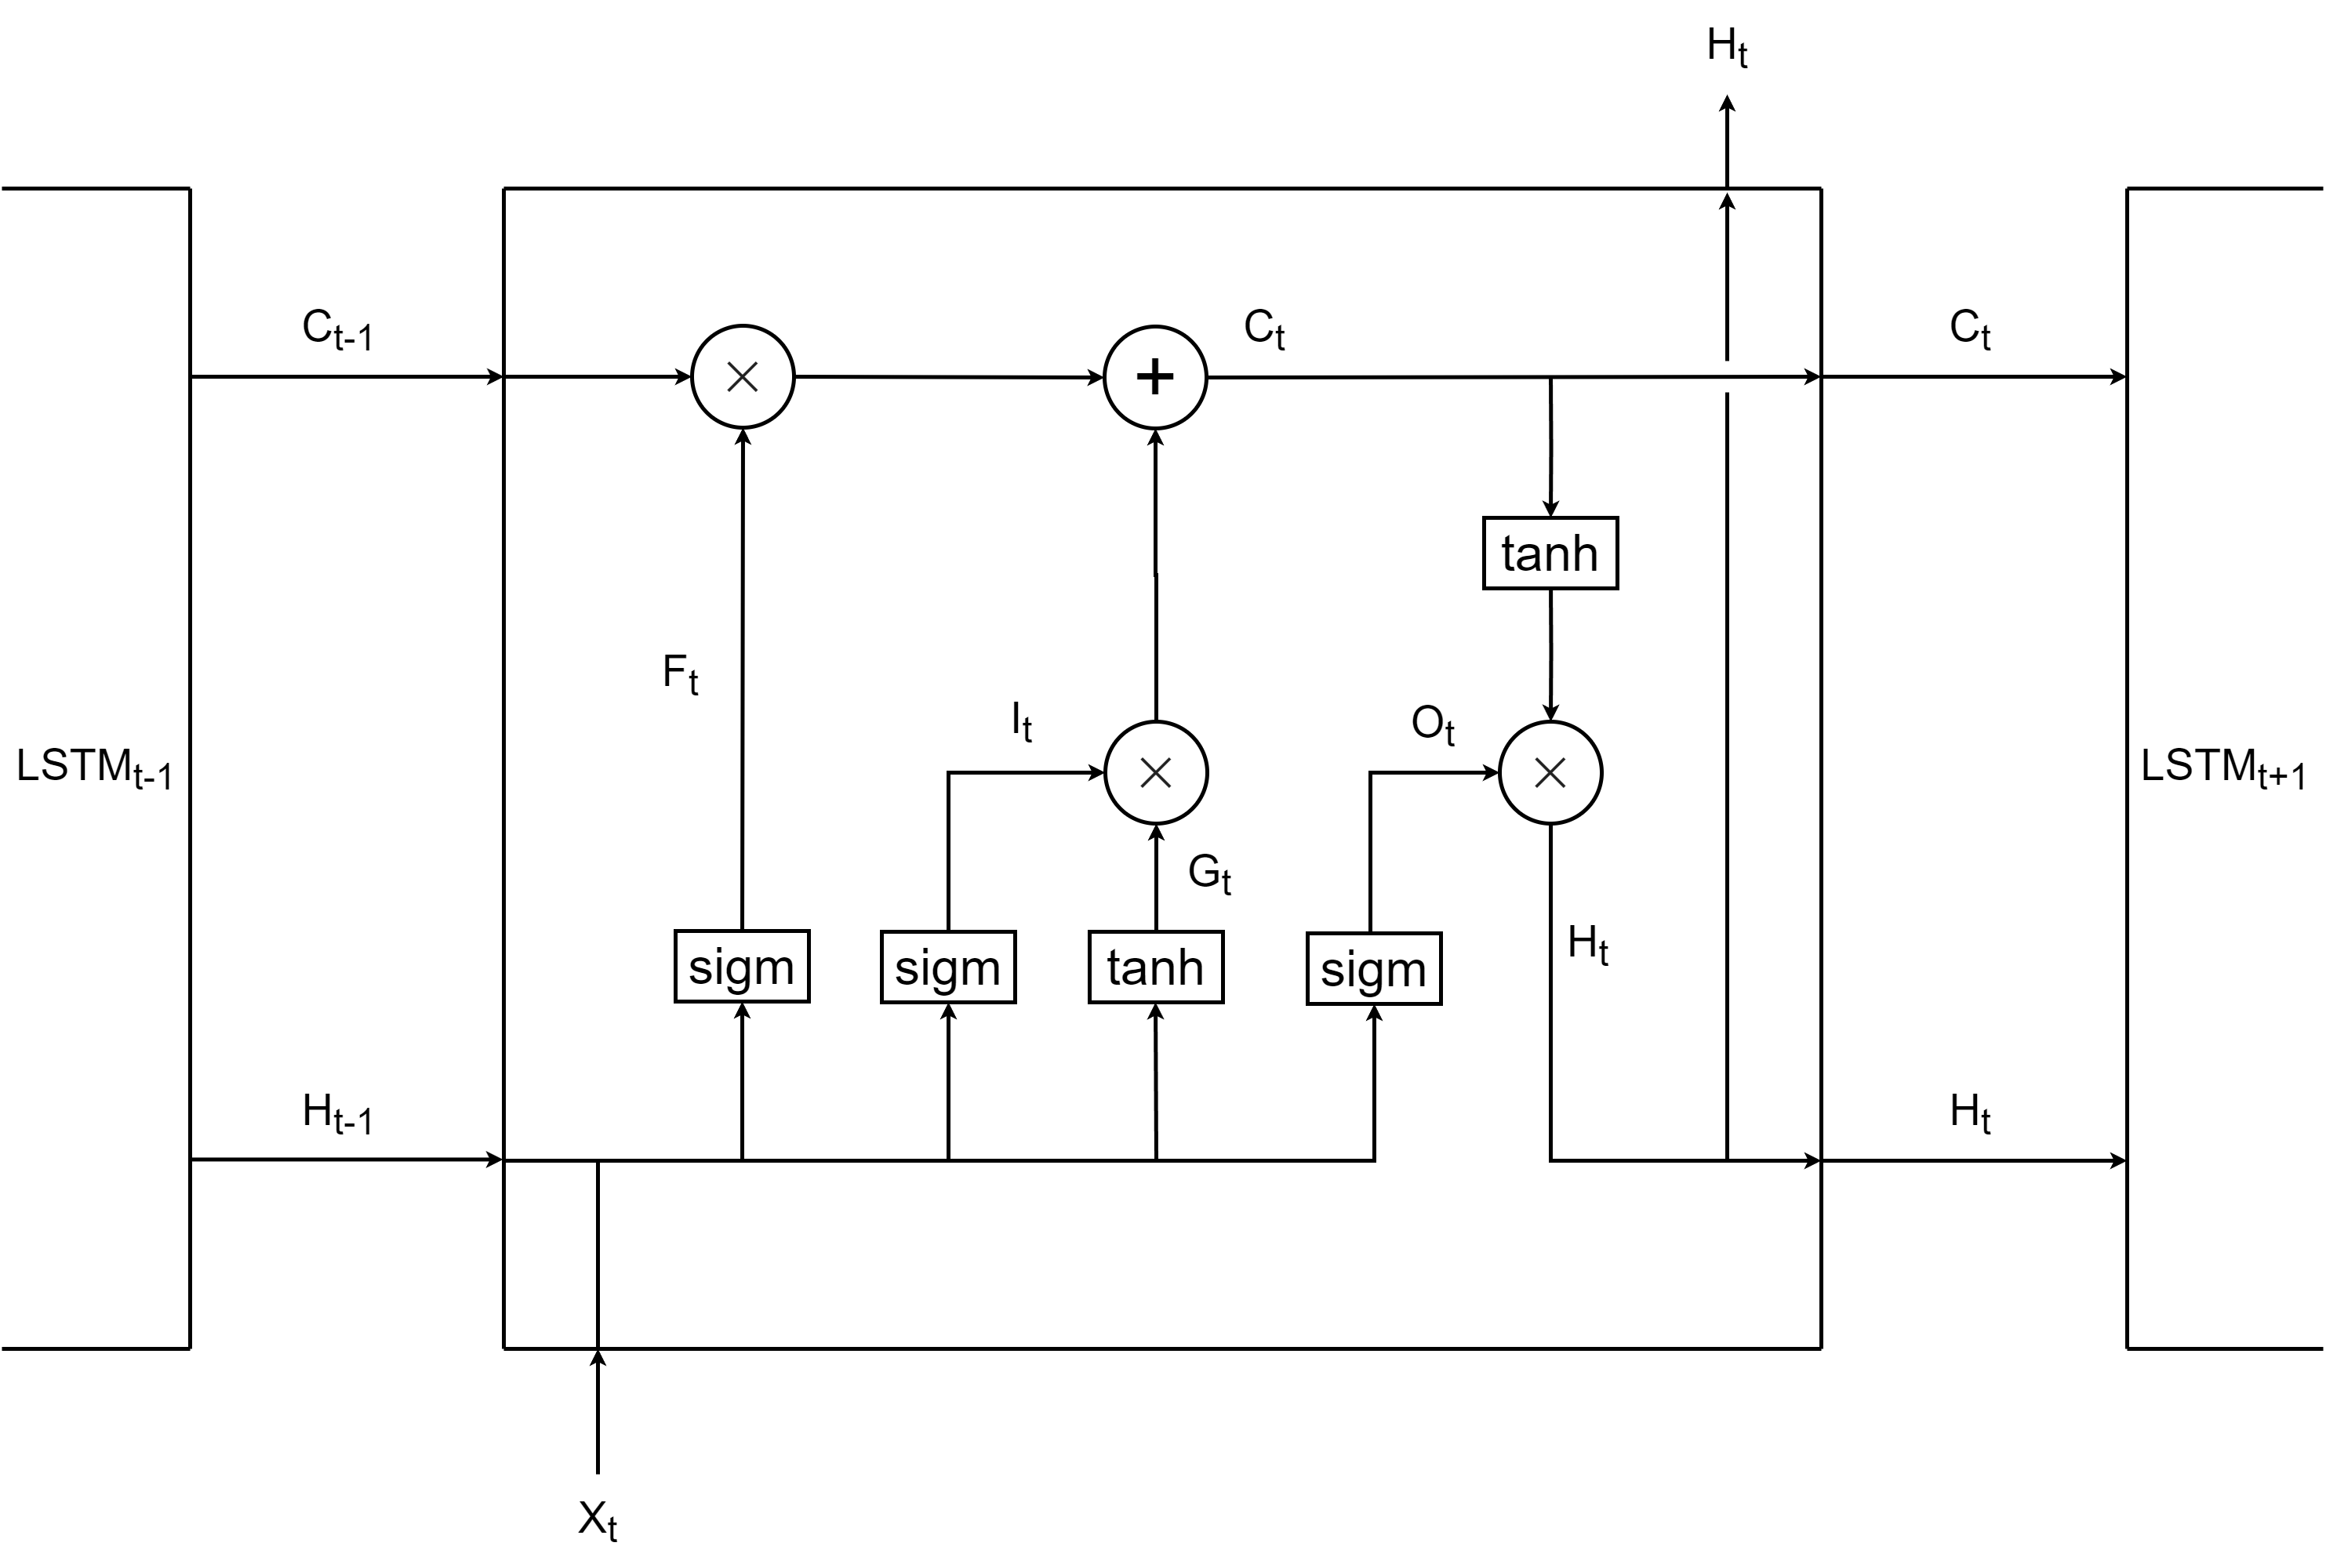
\includegraphics[scale=0.225]{../GMs/Pl2/LSTM.png}
    \caption*{\gostFont Рисунок \thechaptercntr .\theimagecntr \spc {--} Структура ячейки LSTM.}
    \label{fig:LSTM}
  \end{sidewaysfigure} \addtocounter{imagecntr}{1}

  \par \redline Врата забывания ($F_t$) необходимы для исключения некоторый информации из долгосрочной памяти сети ($C_t$) и рассчитываются по формуле (\thechaptercntr .\theformulacntr):

  \formulaspace \par \redline 
    $F_t = sigm(W_f \times X_t + U_f \times H_{t-1} + b_f)$
    \hfill (\thechaptercntr .\theformulacntr) \redline
  \formulaspace \addtocounter{formulacntr}{1}

  \begin{tabular}{p{0,875cm}p{0,3cm}p{15,175cm}}
		& где  & $F_t$ {--} вектор врат забывания; \\
    & 	   & $X_t$ {--} вектор входных значений; \\
		& 	   & $W_f$ {--} матрица весов врат забывания для взаимодействия с входным вектором; \\
    & 	   & $H_{t-1}$ {--} вектор краткосрочной памяти сети на прошлой итерации (из прошлого); \\
    & 	   & $b_f$ {--} вектор смещения для врат забывания; \\
    & 	   & $U_f$ {--} матрица весов врат забывания для взаимодействия с вектором краткосрочной памяти. \\
  \end{tabular}

  \par \redline Врата новой памяти ($G_t$) отвечают за формирование, так скажем, претендентов на новую долгосрочную память ($C_t$) и рассчитываются по формуле (\thechaptercntr .\theformulacntr):

  \formulaspace \par \redline 
    $G_t = tanh(W_g \times X_t + U_g \times H_{t-1} + b_g)$
    \hfill (\thechaptercntr .\theformulacntr) \redline
  \formulaspace \addtocounter{formulacntr}{1}

  \begin{tabular}{p{0,875cm}p{0,3cm}p{15,175cm}}
		& где  & $G_t$ {--} вектор врат новой памяти; \\
		& 	   & $W_g$ {--} матрица весов врат новой памяти для взаимодействия с входным вектором; \\
    & 	   & $b_g$ {--} вектор смещения для врат новой памяти; \\
    & 	   & $U_g$ {--} матрица весов врат новой памяти для взаимодействия с вектором краткосрочной памяти. \\
  \end{tabular}

  \par \redline Врата входа ($I_t$) решают, что из врат новой памяти ($G_t$) сможет попасть в новую долгосрочную память ($C_t$), выполняя тем самым роль отбора, благодаря которой в долгосрочную память сети могут попасть новые зависимости или укрепиться уже имеющиеся. Врата входа рассчитываются по формуле (\thechaptercntr .\theformulacntr):

  \formulaspace \par \redline 
    $I_t = sigm(W_i \times X_t + U_i \times H_{t-1} + b_i)$
    \hfill (\thechaptercntr .\theformulacntr) \redline
  \formulaspace \addtocounter{formulacntr}{1}

  \begin{tabular}{p{0,875cm}p{0,3cm}p{15,175cm}}
		& где  & $I_t$ {--} вектор врат входа; \\
		& 	   & $W_i$ {--} матрица весов врат входа для взаимодействия с входным вектором; \\
    & 	   & $b_i$ {--} вектор смещения для врат входа; \\
    & 	   & $U_i$ {--} матрица весов врат входа для взаимодействия с вектором краткосрочной памяти. \\
  \end{tabular}

  \par \redline Долгосрочная память ($C_t$) хранит в себе особенности и закономерности времного ряда на протяжении всей истории. Наличие такой памяти исключает забывание некоторых особенностей в данных, которые повторяются очень редко или удалены друг от друга на значительном расстонии относительно оси абсцисс. Долгосрочная память рассчитывается по формуле (\thechaptercntr .\theformulacntr):

  \formulaspace \par \redline 
    $C_t = F_t \times C_{t-1} + I_t \times G_t$
    \hfill (\thechaptercntr .\theformulacntr) \redline
  \formulaspace \addtocounter{formulacntr}{1}

  \begin{tabular}{p{0,875cm}p{0,3cm}p{15,175cm}}
		& где  & $C_{t-1}$ {--} вектор долгосрочной памяти сети на прошлой итерации (из прошлого). \\
  \end{tabular}

  \par \redline Врата выхода ($O_t$) контролируют, какая информация из долгосрочной памяти поступит в новую краткосрочную память, и рассчитываются по формуле (\thechaptercntr .\theformulacntr):

  \formulaspace \par \redline 
    $O_t = sigm(W_o \times X_t + U_o \times H_{t-1} + b_o)$
    \hfill (\thechaptercntr .\theformulacntr) \redline
  \formulaspace \addtocounter{formulacntr}{1}

  \begin{tabular}{p{0,875cm}p{0,3cm}p{15,175cm}}
		& где  & $O_t$ {--} вектор врат выхода; \\
		& 	   & $W_o$ {--} матрица весов врат выхода для взаимодействия с входным вектором; \\
    & 	   & $b_o$ {--} вектор смещения для врат выхода; \\
    & 	   & $U_o$ {--} матрица весов врат выхода для взаимодействия с вектором краткосрочной памяти. \\
  \end{tabular}

  \par \redline Краткосрочная память сети хранит в себе закономерности временного ряда в ближайшей его истории. Эта память явяется выходом ячейки LSTM и в дальнейшем непосредственно участвует при составлении прогноза. Новая краткосрочная память сети рассчитывается по формуле: 

  \formulaspace \par \redline 
    $H_t = O_t \times tanh(C_t)$
    \hfill (\thechaptercntr .\theformulacntr) \redline
  \formulaspace \addtocounter{formulacntr}{1}

  \par \redline Теперь необходимо понять, что делать с краткосрочной памятью ячейки LSTM, как с помощью неё получить прогноз? Ответ на этот вопрос весьма прост: для этого можно использовать один обычный нейрон с сигмоидальной функцией активации. Расчёт прогноза производится по формеле (\thechaptercntr .\theformulacntr):

  \formulaspace \par \redline 
    $Y_t = sigm(W_y \times H_t + b_y)$
    \hfill (\thechaptercntr .\theformulacntr) \redline
  \formulaspace \addtocounter{formulacntr}{1}

  \begin{tabular}{p{0,875cm}p{0,3cm}p{15,175cm}}
		& где  & $Y_t$ {--} вектор прогноза; \\
		& 	   & $W_y$ {--} матрица весов врат выхода для взаимодействия с входным краткосрочной памяти; \\
    & 	   & $b_y$ {--} вектор смещения для прогноза.
  \end{tabular}

  \par \redline Таким образом можно получить прогноз, используя сеть LSTM. Теперь, когда точно известно, как можно получить прогноз используя сесть LSTM, приступим к её обучению. 

  \par
}

\subtitlespace

\subsection*{ 
  \gostTitleFont
  \redline
  \thechaptercntr .\thesubchaptercntr \spc 
  Обучение сети LSTM.
} \addtocounter{subchaptercntr}{1} 
  
\subtitlespace
  
{\gostFont

  \par \redline Обучение сети LSTM будет проводиться с помощью метода обратного распространения ошибки во времени. Этот метод позволяет учитывать временные зависимости, благодаря чему можно решить проблему обучения сети с обратными связями. Данный метод предполагает поиск ошибки сети, <<протягиение>> этой ошибки по каждому элементу сети с помощью метода градиентного спуска, после чего обучение весовых коэффицентов. <<Протягивание>> ошибки необходимо, чтобы рассчитать вклад каждого элемента в общую ошибку и изменить величину весового коэффициента в соответствии с ошибкой самого элемента. 

  \par \redline Для определения ошибки самой сети воспользуемся среднеквадратической ошибкой (MSE), которую можно рассчитать по формуле (\thechaptercntr .\theformulacntr):

  \formulaspace \par \redline 
    $MSE = 0.5 \cdot (E_t - Y_t)^2$
    \hfill (\thechaptercntr .\theformulacntr) \redline
  \formulaspace \addtocounter{formulacntr}{1}

  \begin{tabular}{p{0,875cm}p{0,3cm}p{15,175cm}}
		& где  & $Y_t$ {--} вектор прогноза; \\
		& 	   & $E_t$ {--} вектор реальных эталонных значений, говорящий о том, какие значения прогноза должны быть. \\
  \end{tabular}

  \par \redline Определив ошибку сети появляется возможность определить ошибку по выходному нейрону по формуле (\thechaptercntr .\theformulacntr):

  \formulaspace \par \redline 
    $\scaleto{\frac{\delta MSE}{\delta Y_t}}{18pt} = (Y_t - E_t) \times sigm'(Y_t)$
    \hfill (\thechaptercntr .\theformulacntr) \redline
  \formulaspace \addtocounter{formulacntr}{1}

  \begin{tabular}{p{0,875cm}p{0,3cm}p{15,175cm}}
		& где  & $\scaleto{\frac{\delta MSE}{\delta Y_t}}{18pt}$ {--} вектор ошибки выходного нейрона. \\
  \end{tabular}

  \par \redline Теперь появилась возможность определить ошибку по весам матрицы $W_y$ по формуле (\thechaptercntr .\theformulacntr):

  \formulaspace \par \redline 
    $\scaleto{\frac{\delta MSE}{\delta W_y}}{18pt} = \scaleto{\frac{\delta MSE}{\delta Y_y} \times \frac{\delta Y_t}{\delta W_y}}{18pt} = \scaleto{\frac{\delta MSE}{\delta Y_t}}{18pt} \times H_t$
    \hfill (\thechaptercntr .\theformulacntr) \redline
  \formulaspace \addtocounter{formulacntr}{1}

  \begin{tabular}{p{0,875cm}p{0,3cm}p{15,175cm}}
		& где  & $\scaleto{\frac{\delta MSE}{\delta W_y}}{18pt}$ {--} матрица ошибок весовых коэффициентов выходного нейрона. \\
  \end{tabular}

  \par \redline Схожим образом находим ошибку по смещениям выходного нейрона с помощью формулы (\thechaptercntr .\theformulacntr):

  \formulaspace \par \redline 
    $\scaleto{\frac{\delta MSE}{\delta b_y}}{20pt} = \scaleto{\frac{\delta MSE}{\delta Y_y} \times \frac{\delta Y_t}{\delta b_y}}{18pt} = \scaleto{\frac{\delta MSE}{\delta Y_t}}{18pt}$
    \hfill (\thechaptercntr .\theformulacntr) \redline
  \formulaspace \addtocounter{formulacntr}{1}

  \begin{tabular}{p{0,875cm}p{0,3cm}p{15,175cm}}
		& где  & $\scaleto{\frac{\delta MSE}{\delta b_y}}{20pt}$ {--} вектор ошибок коэффициентов смещений выходного нейрона. \\
  \end{tabular}

  \par \redline Для обучения весовых коэффициентов выходного нейрона воспользуемся общей для обучения любых весовых коэффициентов формулой (\thechaptercntr .\theformulacntr), подставив туда необходимые значения:

  \formulaspace \par \redline 
    $W = W - \alpha \cdot \scaleto{\frac{\delta MSE}{\delta W}}{18pt}$
    \hfill (\thechaptercntr .\theformulacntr) \redline
  \formulaspace \addtocounter{formulacntr}{1}

  \begin{tabular}{p{0,875cm}p{0,3cm}p{15,175cm}}
		& где  & $W$ {--} матрица весовых коэффициентов; \\
    & где  & $\scaleto{\frac{\delta MSE}{\delta W}}{20pt}$ {--} матрица ошибок весовых коэффициентов. \\
  \end{tabular}

  \par \redline Для обучения коэффициентов смещения выходного нейрона воспользуемся общей для обучения любых коэффициентов смещений формулой (\thechaptercntr .\theformulacntr), подставив туда необходимые значения:

  \formulaspace \par \redline 
    $b = b + \alpha \cdot \scaleto{\frac{\delta MSE}{\delta b}}{18pt}$
    \hfill (\thechaptercntr .\theformulacntr) \redline
  \formulaspace \addtocounter{formulacntr}{1}

  \par \redline Далее переходим к обучения самой сети. Для этого в первую очередь необходимо определить ошибку краткосрочной памяти. Это можно сделать по формуле (\thechaptercntr .\theformulacntr):

  \formulaspace \par \redline 
    $\scaleto{\frac{\delta MSE}{\delta H_t}}{18pt} = \scaleto{\frac{\delta MSE}{\delta Y_y} \times \frac{\delta Y_t}{\delta H_y}}{18pt} + \scaleto{\frac{\delta MSE}{\delta F_{t+1}} \times \frac{\delta F_{t+1}}{\delta H_y}}{18pt} + \scaleto{\frac{\delta MSE}{\delta I_{t+1}} \times \frac{\delta I_{t+1}}{\delta H_y}}{18pt} + \scaleto{\frac{\delta MSE}{\delta G_{t+1}} \times \frac{\delta G_{t+1}}{\delta H_y}}{18pt} + \scaleto{\frac{\delta MSE}{\delta O_{t+1}} \times \frac{\delta O_{t+1}}{\delta H_y}}{18pt} = \scaleto{\frac{\delta MSE}{\delta Y_t}}{18pt}$
    \hfill (\thechaptercntr .\theformulacntr) \redline
  \formulaspace \addtocounter{formulacntr}{1}

  \begin{tabular}{p{0,875cm}p{0,3cm}p{15,175cm}}
		& где  & $\alpha$ {--} скорость обучения. \\
  \end{tabular}

  \par \redline 

  \par \redline 

%%%%%%%%%%%%%%%%%%%%%%%%%%%%%%%%%%%%%%%%%%%%%%%%%%%%%%%%%%%%%%%%%%%%%%%%%%%%%%%%%%%%%%%%%%%%%%%%%%%%%%%%%%%%%%%%%%%%%%

  \par \redline Ошибку по матрице весовых коэффициентов врат забывания для взаимодействия с входным вектором можно рассчитать по формуле (\thechaptercntr .\theformulacntr):

  \formulaspace \par \redline 
    $\scaleto{\frac{\delta MSE}{\delta W_f}}{18pt} = \scaleto{\frac{\delta MSE}{\delta F_t} \times \frac{\delta F_t}{\delta W_f}}{18pt} = \scaleto{\frac{\delta MSE}{\delta F_t}}{18pt} \times X_t$
    \hfill (\thechaptercntr .\theformulacntr) \redline
  \formulaspace \addtocounter{formulacntr}{1}

  \begin{tabular}{p{0,875cm}p{0,3cm}p{15,175cm}}
		& где  & $\scaleto{\frac{\delta MSE}{\delta W_f}}{18pt}$ {--} ошибка по матрице весовых коэффициентов врат забывания для взаимодействия с входным вектором. \\
  \end{tabular}

  \par \redline Ошибку по матрице весовых коэффициентов врат забывания для взаимодействия с вектором краткосрочной памяти можно рассчитать по формуле (\thechaptercntr .\theformulacntr):

  \formulaspace \par \redline 
    $\scaleto{\frac{\delta MSE}{\delta U_f}}{18pt} = \scaleto{\frac{\delta MSE}{\delta F_t} \times \frac{\delta F_t}{\delta U_f}}{18pt} = \scaleto{\frac{\delta MSE}{\delta F_t}}{18pt} \times H_{t-1}$
    \hfill (\thechaptercntr .\theformulacntr) \redline
  \formulaspace \addtocounter{formulacntr}{1}

  \begin{tabular}{p{0,875cm}p{0,3cm}p{15,175cm}}
		& где  & $\scaleto{\frac{\delta MSE}{\delta U_f}}{18pt}$ {--} ошибка по матрице весовых коэффициентов врат забывания для взаимодействия с вектором краткосрочной памяти. \\
  \end{tabular}

  \par \redline Обучить весовые коэффициенты матриц врат забывания можно, подставив соответствующие значения в формулу (\thechaptercntr .12).

  \par \redline Ошибка по вектору смещений врат забывания определяется по формуле (\thechaptercntr .\theformulacntr):

  \formulaspace \par \redline 
    $\scaleto{\frac{\delta MSE}{\delta b_f}}{20pt} = \scaleto{\frac{\delta MSE}{\delta F_t} \times \frac{\delta F_t}{\delta b_f}}{18pt} = \scaleto{\frac{\delta MSE}{\delta F_t}}{18pt}$
    \hfill (\thechaptercntr .\theformulacntr) \redline
  \formulaspace \addtocounter{formulacntr}{1}

  \par \redline Обучить коэффициенты смещения врат забывания можно, подставив соответствующие значения в формулу (\thechaptercntr .13).

%%%%%%%%%%%%%%%%%%%%%%%%%%%%%%%%%%%%%%%%%%%%%%%%%%%%%%%%%%%%%%%%%%%%%%%%%%%%%%%%%%%%%%%%%%%%%%%%%%%%%%%%%%%%%%%%%%%%%%

  \par \redline Ошибку по матрице весовых коэффициентов врат входа для взаимодействия с входным вектором можно рассчитать по формуле (\thechaptercntr .\theformulacntr):

  \formulaspace \par \redline 
    $\scaleto{\frac{\delta MSE}{\delta W_i}}{18pt} = \scaleto{\frac{\delta MSE}{\delta I_t} \times \frac{\delta I_t}{\delta W_i}}{18pt} = \scaleto{\frac{\delta MSE}{\delta I_t}}{18pt} \times X_t$
    \hfill (\thechaptercntr .\theformulacntr) \redline
  \formulaspace \addtocounter{formulacntr}{1}

  \begin{tabular}{p{0,875cm}p{0,3cm}p{15,175cm}}
		& где  & $\scaleto{\frac{\delta MSE}{\delta W_i}}{18pt}$ {--} ошибка по матрице весовых коэффициентов врат входа для взаимодействия с входным вектором. \\
  \end{tabular}

  \par \redline Ошибку по матрице весовых коэффициентов врат входа для взаимодействия с вектором краткосрочной памяти можно рассчитать по формуле (\thechaptercntr .\theformulacntr):

  \formulaspace \par \redline 
    $\scaleto{\frac{\delta MSE}{\delta U_i}}{18pt} = \scaleto{\frac{\delta MSE}{\delta I_t} \times \frac{\delta I_t}{\delta U_i}}{18pt} = \scaleto{\frac{\delta MSE}{\delta I_t}}{18pt} \times H_{t-1}$
    \hfill (\thechaptercntr .\theformulacntr) \redline
  \formulaspace \addtocounter{formulacntr}{1}

  \begin{tabular}{p{0,875cm}p{0,3cm}p{15,175cm}}
		& где  & $\scaleto{\frac{\delta MSE}{\delta U_i}}{18pt}$ {--} ошибка по матрице весовых коэффициентов врат входа для взаимодействия с вектором краткосрочной памяти. \\
  \end{tabular}

  \par \redline Обучить весовые коэффициенты матриц врат входа можно, подставив соответствующие значения в формулу (\thechaptercntr .12).

  \par \redline Ошибка по вектору смещений врат входа определяется по формуле (\thechaptercntr .\theformulacntr): 

  \formulaspace \par \redline 
    $\scaleto{\frac{\delta MSE}{\delta b_i}}{20pt} = \scaleto{\frac{\delta MSE}{\delta I_t} \times \frac{\delta I_t}{\delta b_i}}{18pt} = \scaleto{\frac{\delta MSE}{\delta I_t}}{18pt}$
    \hfill (\thechaptercntr .\theformulacntr) \redline
  \formulaspace \addtocounter{formulacntr}{1}

  \par \redline Обучить коэффициенты смещения врат входа можно, подставив соответствующие значения в формулу (\thechaptercntr .13).

%%%%%%%%%%%%%%%%%%%%%%%%%%%%%%%%%%%%%%%%%%%%%%%%%%%%%%%%%%%%%%%%%%%%%%%%%%%%%%%%%%%%%%%%%%%%%%%%%%%%%%%%%%%%%%%%%%%%%%

  \par \redline Ошибку по матрице весовых коэффициентов врат новой памяти для взаимодействия с входным вектором можно рассчитать по формуле (\thechaptercntr .\theformulacntr):

  \formulaspace \par \redline 
    $\scaleto{\frac{\delta MSE}{\delta W_g}}{18pt} = \scaleto{\frac{\delta MSE}{\delta G_t} \times \frac{\delta G_t}{\delta W_g}}{18pt} = \scaleto{\frac{\delta MSE}{\delta G_t}}{18pt} \times X_t$
    \hfill (\thechaptercntr .\theformulacntr) \redline
  \formulaspace \addtocounter{formulacntr}{1}

  \begin{tabular}{p{0,875cm}p{0,3cm}p{15,175cm}}
		& где  & $\scaleto{\frac{\delta MSE}{\delta W_g}}{18pt}$ {--} ошибка по матрице весовых коэффициентов врат новой памяти для взаимодействия с входным вектором. \\
  \end{tabular}

  \par \redline Ошибку по матрице весовых коэффициентов врат новой памяти для взаимодействия с вектором краткосрочной памяти можно рассчитать по формуле (\thechaptercntr .\theformulacntr):

  \formulaspace \par \redline 
    $\scaleto{\frac{\delta MSE}{\delta U_g}}{18pt} = \scaleto{\frac{\delta MSE}{\delta G_t} \times \frac{\delta G_t}{\delta U_g}}{18pt} = \scaleto{\frac{\delta MSE}{\delta G_t}}{18pt} \times H_{t-1}$
    \hfill (\thechaptercntr .\theformulacntr) \redline
  \formulaspace \addtocounter{formulacntr}{1}

  \begin{tabular}{p{0,875cm}p{0,3cm}p{15,175cm}}
		& где  & $\scaleto{\frac{\delta MSE}{\delta U_g}}{18pt}$ {--} ошибка по матрице весовых коэффициентов врат новой памяти для взаимодействия с вектором краткосрочной памяти. \\
  \end{tabular}

  \par \redline Обучить весовые коэффициенты матриц врат новой памяти можно, подставив соответствующие значения в формулу (\thechaptercntr .12).

  \par \redline Ошибка по вектору смещений врат новой памяти определяется по формуле (\thechaptercntr .\theformulacntr):

  \formulaspace \par \redline 
    $\scaleto{\frac{\delta MSE}{\delta b_g}}{20pt} = \scaleto{\frac{\delta MSE}{\delta G_t} \times \frac{\delta G_t}{\delta b_g}}{18pt} = \scaleto{\frac{\delta MSE}{\delta G_t}}{18pt}$
    \hfill (\thechaptercntr .\theformulacntr) \redline
  \formulaspace \addtocounter{formulacntr}{1}

  \par \redline Обучить коэффициенты смещения врат новой памяти можно, подставив соответствующие значения в формулу (\thechaptercntr .13).

%%%%%%%%%%%%%%%%%%%%%%%%%%%%%%%%%%%%%%%%%%%%%%%%%%%%%%%%%%%%%%%%%%%%%%%%%%%%%%%%%%%%%%%%%%%%%%%%%%%%%%%%%%%%%%%%%%%%%%

  \par \redline Ошибку по матрице весовых коэффициентов врат выхода для взаимодействия с входным вектором можно рассчитать по формуле (\thechaptercntr .\theformulacntr):

  \formulaspace \par \redline 
    $\scaleto{\frac{\delta MSE}{\delta W_o}}{18pt} = \scaleto{\frac{\delta MSE}{\delta O_t} \times \frac{\delta O_t}{\delta W_o}}{18pt} = \scaleto{\frac{\delta MSE}{\delta O_t}}{18pt} \times X_t$
    \hfill (\thechaptercntr .\theformulacntr) \redline
  \formulaspace \addtocounter{formulacntr}{1}

  \begin{tabular}{p{0,875cm}p{0,3cm}p{15,175cm}}
		& где  & $\scaleto{\frac{\delta MSE}{\delta W_g}}{18pt}$ {--} ошибка по матрице весовых коэффициентов врат новой памяти для взаимодействия с входным вектором. \\
  \end{tabular}

  \par \redline Ошибку по матрице весовых коэффициентов врат выхода для взаимодействия с вектором краткосрочной памяти можно рассчитать по формуле (\thechaptercntr .\theformulacntr):

  \formulaspace \par \redline 
    $\scaleto{\frac{\delta MSE}{\delta U_o}}{18pt} = \scaleto{\frac{\delta MSE}{\delta O_t} \times \frac{\delta O_t}{\delta U_o}}{18pt} = \scaleto{\frac{\delta MSE}{\delta G_t}}{18pt} \times H_{t-1}$
    \hfill (\thechaptercntr .\theformulacntr) \redline
  \formulaspace \addtocounter{formulacntr}{1}

  \begin{tabular}{p{0,875cm}p{0,3cm}p{15,175cm}}
		& где  & $\scaleto{\frac{\delta MSE}{\delta U_o}}{18pt}$ {--} ошибка по матрице весовых коэффициентов врат выхода для взаимодействия с вектором краткосрочной памяти. \\
  \end{tabular}

  \par \redline Обучить весовые коэффициенты матриц врат выхода можно, подставив соответствующие значения в формулу (\thechaptercntr .12).

  \par \redline Ошибка по вектору смещений врат выхода определяется по формуле (\thechaptercntr .\theformulacntr):

  \formulaspace \par \redline 
    $\scaleto{\frac{\delta MSE}{\delta b_o}}{20pt} = \scaleto{\frac{\delta MSE}{\delta O_t} \times \frac{\delta O_t}{\delta b_o}}{18pt} = \scaleto{\frac{\delta MSE}{\delta O_t}}{18pt}$
    \hfill (\thechaptercntr .\theformulacntr) \redline
  \formulaspace \addtocounter{formulacntr}{1}

  \par \redline Обучить коэффициенты смещения врат выхода можно, подставив соответствующие значения в формулу (\thechaptercntr .13).

%%%%%%%%%%%%%%%%%%%%%%%%%%%%%%%%%%%%%%%%%%%%%%%%%%%%%%%%%%%%%%%%%%%%%%%%%%%%%%%%%%%%%%%%%%%%%%%%%%%%%%%%%%%%%%%%%%%%%%

  \par \redline 

  \par
}

\setcounter{subchaptercntr}{1}
\setcounter{formulacntr}{1}
\setcounter{imagecntr}{1}
